%%%%%%%%%%%%%%%%%%%%%%%%%%%%%%%%%%%%%%%%%
% University/School Laboratory Report
% LaTeX Template
% Version 3.1 (25/3/14)
%
% This template has been downloaded from:
% http://www.LaTeXTemplates.com
%
% Original author:
% Linux and Unix Users Group at Virginia Tech Wiki 
% (https://vtluug.org/wiki/Example_LaTeX_chem_lab_report)
%
% License:
% CC BY-NC-SA 3.0 (http://creativecommons.org/licenses/by-nc-sa/3.0/)
%
%%%%%%%%%%%%%%%%%%%%%%%%%%%%%%%%%%%%%%%%%

%----------------------------------------------------------------------------------------
%	PACKAGES AND DOCUMENT CONFIGURATIONS
%----------------------------------------------------------------------------------------

\documentclass[12pt]{article}
%\documentclass[14pt]{extarticle}

\usepackage{setspace} % For set space
\usepackage{algorithm} % For pseudo code
\usepackage[noend]{algpseudocode}
\usepackage{siunitx} % Provides the \SI{}{} and \si{} command for typesetting SI units
\usepackage{graphicx} % Required for the inclusion of images
\usepackage{amsmath} % Required for some math elements 
\usepackage{cite} % For citation
\usepackage{algpseudocode}
\usepackage{graphicx}
\usepackage{subfigure}

\setlength\parindent{0pt} % Removes all indentation from paragraphs
\setlength{\parskip}{0.5em}

\renewcommand{\labelenumi}{\alph{enumi}.} % Make numbering in the enumerate environment by letter rather than number (e.g. section 6)
\renewcommand{\baselinestretch}{1.2}
%\usepackage{times} % Uncomment to use the Times New Roman font

%----------------------------------------------------------------------------------------
%	DOCUMENT INFORMATION
%----------------------------------------------------------------------------------------

\title{\large Multiple AI Competition in Self Developed Game \\ Term 2 Report \\ ESTR4998/4999} % Title

\date{\today} % Date for the report

\begin{document}


\maketitle % Insert the title, author and date

\begin{center}
\begin{tabular}{l r}
Partners: & XIAO Tianyi \\ % Partner names
& LUO Lu \\
Instructor: & Prof. Andrej Bogdanov % Instructor/supervisor
\end{tabular}
\end{center}
\newpage


%----------------------------------------------------------------------------------------
%	SECTION 1
%----------------------------------------------------------------------------------------

\begin{abstract}
	We face huge challenge due to the difficulty and complexity of reinforcement learning. So we implement single player mode at first, which is successful. And then we try our best to train 1v1 mode with DQN. Basically, the agents trained with DQN could play our game with logic, like chasing for the ball and making goals. However many problems are found, like the inefficiency of reinforcement learning, and imbalance of a pair of players.
\end{abstract}
 
%----------------------------------------------------------------------------------------
%	SECTION 2
%---------------------------------------------------------------------------------------
\section{Background}

\subsection{Basic Theory}
In our last report, we have provided theories of reinforcement learning, $Q$-learning and Deep $Q$-learning and pseudo codes for them. In this part, in order to make the report easier to understand, we will provide pseudo codes and intuitive descriptions for these algorithms, and the advantages and disadvantages will not be discussed this time.
\subsubsection{$Q$-Learning}
The pseudo code of $Q$-learning is shown as Algorithm 1:
\begin{algorithm}
    \caption{Reinforcement Learning (Zoph et al, 31) }\label{euclid}
    \begin{algorithmic}[1]
    \Require $\gamma$, $\alpha$
    \State Initialize $Q$ (e.g. $Q(s,a) = 0 \ for \ \forall s \in S, \forall a \in A$)
    \For{each episode}
        \State Modify $\alpha$ and $\gamma$
        \State $s \in S$ is initialized as the starting state
        \Repeat
            \State choose a random action or the best action $a \in A(s)$ based on the exploration strategy.
            \State perform action $a$
            \State observe the new state $s'$ and received reward $r$
            \State \small $Q_{k+1}(s, a) = Q_{k}(s, a) + \alpha(r + \gamma \cdot max_{a' \in A(s')}Q_k(s,a') - Q_k(s, a))$
            \State using the experience $\left\langle s,a,r,s'\right\rangle $
            \State $s := s'$
        \Until $s'$ is a goal state or $t$ reaches the limitation
    \EndFor
    \end{algorithmic}
\end{algorithm}

The core of $Q$-learning is that we use a table, $Q$-table, as the memory to identify states of environment and remember the performance of every action in every state. The procedure of training the agent is the procedure to adjust its memory.

The performance of an action is the expected reward if we choose this action. Therefore, the term $max_{a'\in A(s')}Q_k(s,a')$ is the optimal expected reward of the next state, which represents the future reward. $\gamma$, as the discount factor, represents the magnitude of the 'future'. Larger $\gamma$ will make an agent consider in longer-range because the importance of the future will be higher. $\alpha$ is the learning rate, an agent will change the memory faster with higher learning rate, but it may not be great if the learning rate is too high or too low, because we may 'discard' too much previous memory or cannot learning almost anything.

\subsubsection{Deep $Q$-Learning}

The algorithm of DQN is:
\begin{algorithm}[H]
    \caption{Deep $Q$-Network(Mnih et al)}\label{euclid}
    \begin{algorithmic}[1]
    \State Setup replay memory $D$ to capacity $N$
    \State Initialize action-value function $Q$ with random weights $\theta$
    \State Initialize target action-value function $\hat{Q}$ with weights $\theta'$
    \For{each episode}
        \State Initialize sequence $s_1 = {x_1}$ and preprocessed sequence $\phi_1 = \phi(s_1)$
        \State $t := 1$
        \Repeat
            \State Choose a random action or the best action $a_t \in A(s)$ based on the exploration strategy.
            \State Perform action $a_t$
            \State Observe the new input $x_{t+1}$ and received reward $r_t$
            \State Set $s_{t+1} = s_t,a_t,x_{t+1}$ and preprocess $\phi_{t+1} = \phi(s_{t+1})$
            \State Store the experience $(\phi_t, a_t, r_t, \phi_{t+1})$ in $D$
            \State Sample random minibatch of transitions $(\phi_j, a_j, r_j, \phi_{j+1})$ in $D$
            \State Set $y_j = r_j + \gamma max_{a'} \hat{Q}(\phi_{j+1},a'; \theta')$
            \State Perform a gradient descent step on $(y_j - Q(\phi_j, a_j; \theta))^2$ with respect to the network parameters $\theta$
            \State Every C steps reset $\hat{Q} = Q$ 
        \Until $s'$ is a goal state or $t$ reaches the limitation
    \EndFor
    \end{algorithmic}
\end{algorithm}

The core of D$Q$N is similar to $Q$-learning, which is to train a estimator to judge the performance of actions. The difference is that the estimator in $Q$-learning is a memory table but the estimator in D$Q$N is a function with game states as input.

According to previous research, a neural net can approximate any computable function(Wang, 2003), so we can use neural network to approximate the estimate function. In this way, we can train the model in deep learning algorithm to obtain the function without any knowledge about the function itself.

\subsection{Previous Progress}
In the last semester, we have implemented the preliminary version of the game environment and $Q$-Learning agent. In this section, we will briefly reiterate our previous progress before introducing new progress and our opinions.
\subsubsection{Environment}
When we started to draft our proposal, original considerations for designing our environment included complexity, scalability and implemental difficulty. We hoped to design an environment which is easy to implement, complex enough to distinguish the power of different algorithms and can be reused for different game modes, including 1 player, 1 versus 1, and multi-players against multi-players.

Therefore, we designed a game similar to football, and the graph user interface for 1 versus 1 version can be found in figure 1. In this environment, each agent controls one player which is represented as a blue(team 0) or an orange(team 1) rounded rectangle. And the purpose of players is to shoot the ball, which is represented as a white ball, to goal of opponent team, which is represent as white rectangle in the left border(for team 0) and right border(for team 1).

The environment can output a list to represent the game state. For 1 versus 1 mode, the list will contain the position of the current player, the position of the opponent player and the position of the ball.

The environment can receive a list with size equal 2 from a player as input, the first element represents the direction and the second element represents the action, shoot or not. 

After receiving an action, we can call the reward function to calculate the reward of the given action, and return the reward as a scalar number to that agent.

\subsubsection{Agent}

In the last semester, we have finished the design of Q-Learning agent by following the algorithm provided in the background theory section. Moreover, our conclusion of the last term is that our game is too complicated to be trained by Q-Learning even for 1 vs 1 mode, even if we simplified input states.

The reason to simplify states is that the number of raw game states is an enormous figure even without considering the action space. The simplify function will replace the positions of opponent player and ball by logarithms of relative positions(distances) with base 10, which will compress the range of these 4 parameters from several hundred to 7. This will significantly reduce the size of Q-Table and make some simpler situations trainable, and we will discuss this later.


%----------------------------------------------------------------------------------------
%	SECTION 3
%----------------------------------------------------------------------------------------

\section{Implementation}

\subsection{Single Player Mode}
In the beginning stage of our project in this term, we found that it's hard to train AI to play our game with DQN. So to simplify the issue and solve our prolem better, we first implement a single player mode. Then with the experience from single player mode, we are finally able to train DQN AI that could play 1v1 mode with logic.

In this mode, we randomize the initialization of our player and ball. They will be put on the soccer field randomly when each episode begins. And once the player shoot the ball in a door, no matter right door or not, the current episode would end and a new episode of game would start.
\begin{figure}[H]
	\begin{center}
		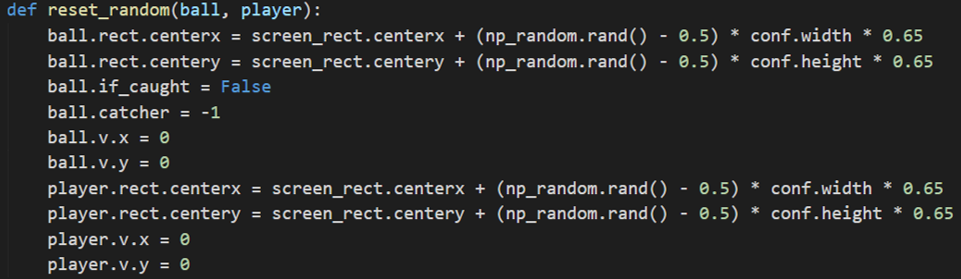
\includegraphics[width=0.9\textwidth]{reset_random}
		\caption{implementation of reset\_random}
	\end{center}
\end{figure}


\subsection{Agent State}
The state of agent represent the features sent to neural network. We add one more item into the agent state, which shows if the player is catching the ball or not. In the soccer game, there is cool down time for each player to prevent it to get the ball back as soon as it just shoots the ball. Therefore the coincidence of positions of player and ball doesn't mean that player could catch and shoot the ball. So one more item in agent state could help AI better understand its situation.


\subsection{Reward Function}
Reward function is crucial in reinforcement learning. As a soccer game, when a team get a goal, it will get huge reward. Besides, when a player catch a ball, it will also recive reward. Besides, to encourage player to keep the ball longer, once the player shoot the ball, it will get punishment.\\
However, only these basic rewards are not enough for training. Below are our modification for other part of reward function.

\subsubsection{Original Reward Function}
 In our original reward function, we give reward to the agent if it's closer to the ball than other player. Otherwise, the agent would get punishment. Besides, if the ball get closer to one door, the team attacking this door would get reward, and other team would get punishment.

\begin{algorithm}[!h]
	\caption{Original Reward$(Agent1,Agent2,Ball)$}
	\begin{algorithmic}
		\State Closer\_Agent(Agent1, Agent2, Ball).reward $+=$ 200
		\State Further\_Agent(Agent1, Agent2, Ball).reward $-=$ 200
		\If {Ball Moves right}
		\State Agent1.reward $+=$ 600
		\State Agent2.reward $-=$ 600
		\EndIf
		\If {Ball Moves left}
		\State Agent2.reward $+=$ 600
		\State Agent1.reward $-=$ 600
		\EndIf
		\If {Ball goes into right door}
		\State Agent1.reward $+=$ 100000
		\State Agent2.reward $-=$ 10000
		\EndIf
		\If {Ball goes into left door}
		\State Agent2.reward $+=$ 100000
		\State Agent1.reward $-=$ 10000
		\EndIf
		\If {Agent shoot the ball}
		\State Agent-shoot-ball.reward $-=$ 1000
		\EndIf
	\end{algorithmic}
\end{algorithm}

\subsubsection{Reward Function For Single Mode}
With Single Player Mode, we need a new reward function. This one is simple. If the player is moving closer to the ball, it will get reward, otherwise it will get punishment. Also, if the player shoot the ball to the direction to the right door, it will get reward. But if it shoots to wrong direction, it will get punishment. Then to encourage the player to keep the ball, it will also have reward when it keeps the ball.

\begin{algorithm}[!h]
	\caption{Single Mode Reward$(Agent,Ball)$}
	\begin{algorithmic}
		\If {Closer(Agent, Ball) or Keep(Agent, Ball)}
		\State Agent.reward $+=$ 200
		\Else
		\State Agent.reward $-=$ 200
		\EndIf
		\If {Ball goes into right door}
		\State Agent.reward $+=$ 100000
		\EndIf
		\If {Ball goes into left door}
		\State Agent.reward $-=$ 10000
		\EndIf
		\If {Agent shoot the ball}
		\State team-of-the-agent.reward $-=$ 1000
		\EndIf
	\end{algorithmic}
\end{algorithm}

\subsubsection{New Reward Function}

Then, with experience from single player mode, we try to modify our original reward function. We cancel the comparison of distance to ball between two agents, instead we only care if the agent is closer to the ball. Also, we cancel some punishment to avoid agent playing to negatively. And we adjust the amount of reward during our test.
\begin{algorithm}[H]
	\caption{New Reward$(Agent1,Agent2,Ball)$}
	\begin{algorithmic}
		\If {Closer(Agent1, Ball)}
		\State Agent1.reward $+=$ 100
		\Else
		\State Agent1.reward $-=$ 100
		\EndIf
		\If {Closer(Agent2, Ball)}
		\State Agent2.reward $+=$ 100
		\Else
		\State Agent2.reward $-=$ 100
		\EndIf
		\If {Ball Moves right}
		\State Agent1.reward $+=$ 100
		\EndIf
		\If {Ball Moves left}
		\State Agent2.reward $+=$ 100
		\EndIf
		\If {Ball goes into right door}
		\State Agent1.reward $+=$ 100000
		\State Agent2.reward $-=$ 10000
		\EndIf
		\If {Ball goes into left door}
		\State Agent2.reward $+=$ 100000
		\State Agent1.reward $-=$ 10000
		\EndIf
		\If {Agent shoot the ball}
		\State Agent-shoot-ball.reward $-=$ 1000
		\EndIf
	\end{algorithmic}
\end{algorithm}

\subsection{Neural Network}
In the implementation of our DQN, we look through a good tutorial of MorvanZhou(Zhou), which help us a lot. And we use two DQN implementation in our project, one offered in the tutorial, and another one implemented by us with keras, inspired by previous version, referenced from tutorial. Below we will use the second implementation, to briefly introduce our neural network. However for our experiment, since the training of keras is appearently slower than tensorflow, so we use first implementation to collect the data.

\subsubsection{Structrue of Nerual Network}
There are two layers in our nerual network. In the first layer, we add a relu activation layer in the end. All variables are initialized with random normal initializers.
\begin{figure}[H]
	\begin{center}
		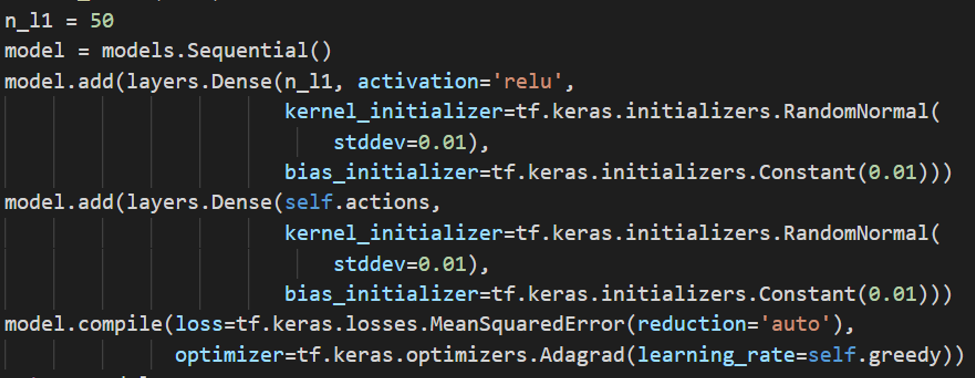
\includegraphics[width=0.9\textwidth]{network}
		\caption{structure of nerual network}
	\end{center}
\end{figure}

\subsubsection{Update}
We randomly pick batch of memory, and calculate their actions from previous state to target network, and after state to eval network. Then we calculate relative q values of target model, and update the parameters in eval network. Also, the parameters in target network will be updated every R rounds of update.(R=300 in our project).
\begin{figure}[H]
	\begin{center}
		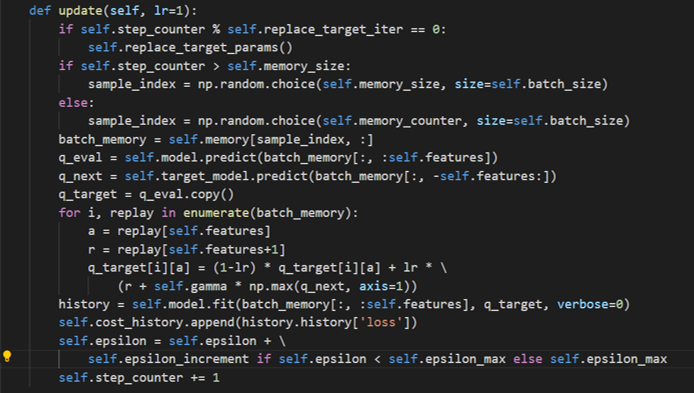
\includegraphics[width=0.9\textwidth]{update}
		\caption{update}
	\end{center}
\end{figure}

\subsection{Measurement of Performance}
In the reference tutorial of reinforcement learning, the cost was used to measure the performance of DQN, which is quite a bad measurement in fact. Therefore, in our project, we use the q-values and average reward as measurements of our performances. We record the value of action we choose to form the history of q-values. And for every 100 steps, we sum up the rewards of 100 steps and calculate the average reward.


%----------------------------------------------------------------------------------------
%	SECTION 4
%----------------------------------------------------------------------------------------

\section{Result}

In this section, we will show our result in two different modes.

\subsection{Single Player Mode}

In the single player mode, we use both Q-learning and DQN to train our agent. Although according to our previous conclusion, Q-learning can not play very complicated game, however with one less player, the relative complexity of Q-table also reduce a lot. Therefore we decide to also use Q-learning in the single player mode.

\begin{figure}[htbp]
	\centering
	\subfigure[DQN]{
		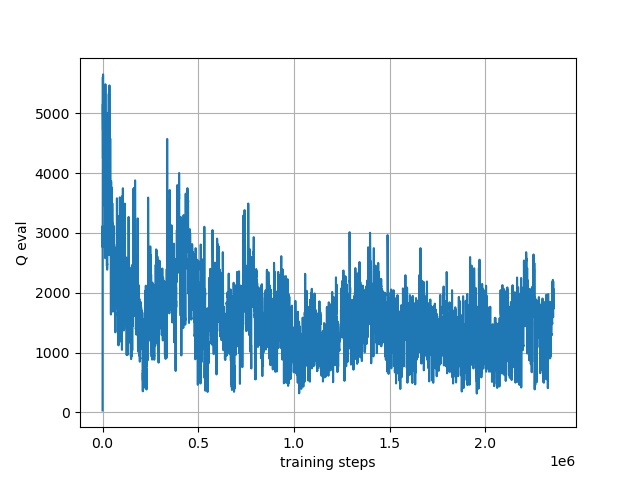
\includegraphics[width=6cm]{qvalue-1-DQN.jpg}
	}
	\subfigure[Q-learning]{
		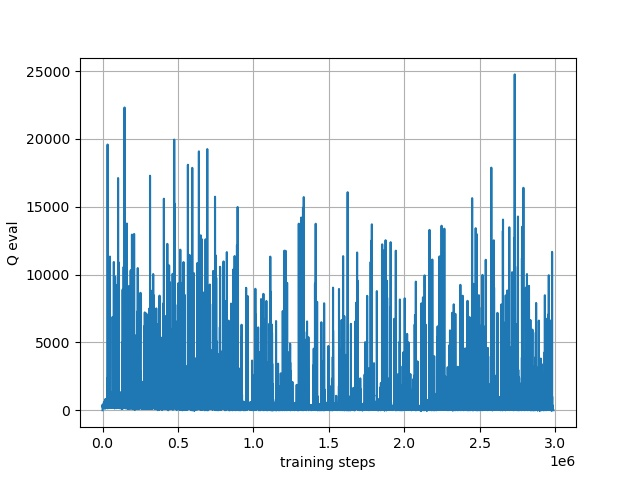
\includegraphics[width=6cm]{qvalue-1-QL.jpg}
	}
	\caption{Q-values in single mode}
\end{figure}
\begin{figure}[htbp]
	\centering
	\subfigure[DQN]{
		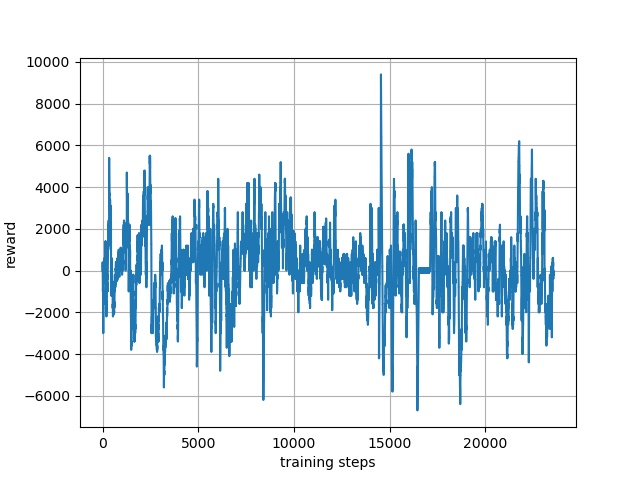
\includegraphics[width=6cm]{reward-1-DQN.jpg}
	}
	\subfigure[Q-learning]{
		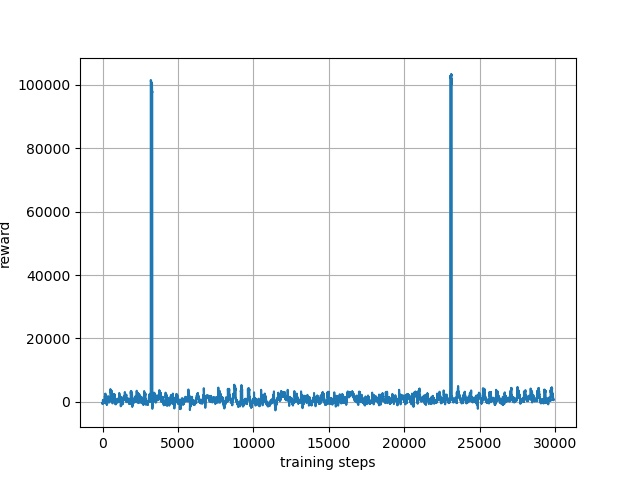
\includegraphics[width=6cm]{reward-1-QL.jpg}
	}
	\caption{rewards in single mode}
\end{figure}

Comparing two Q-values figures, we can find thay there is an appearent decline in DQN, but for Q-learning, the distribution of Q-values seems more random. And for average rewards, the waves in DQN is much more significant compared with Q-learning.

However, these 2 measurement are not that accurate for measuring performance. So, we use make a test on the DQN and Q-learning agent. We test how many how many score they can get in 100 episodes of game.

\begin{figure}[htbp]
	\centering
	\subfigure[DQN-73/100]{
		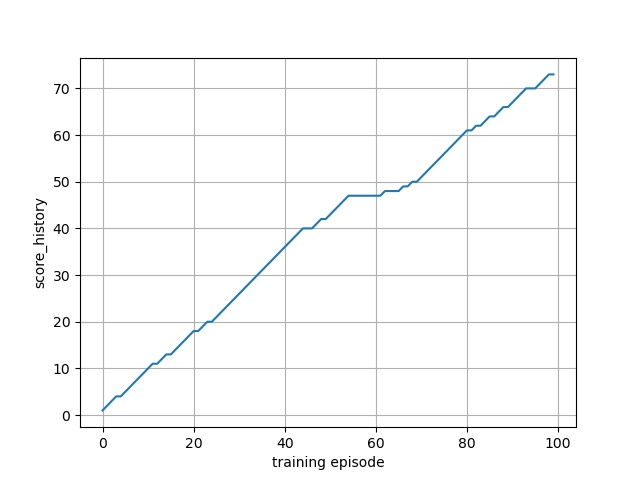
\includegraphics[width=6cm]{score-1-DQN-73.jpg}
	}
	\subfigure[Q-learning-51/100]{
		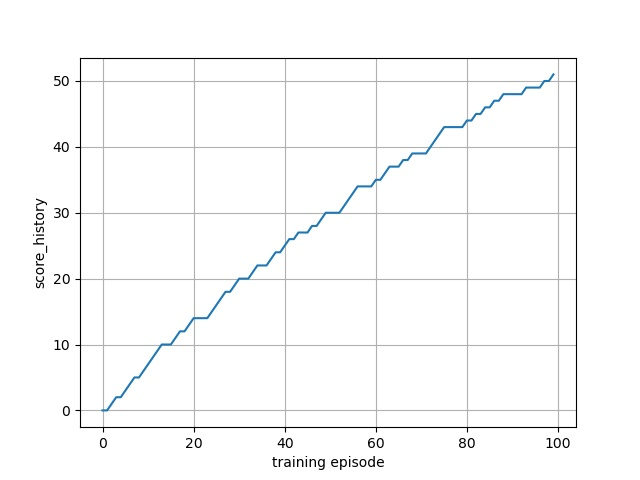
\includegraphics[width=6cm]{score-1-QL-51.jpg}
	}
	\caption{total score for 100 round in single mode}
\end{figure}

 The result shows that both DQN and Q-learning can play the game with logic, since the score they get are appearntly higher than a random player. And the performance of DQN (73 in 100 scores) is higher than Q-learning(51 in 100 scores), which could prove that DQN is more powerful than Q-learning.


\subsection{1v1 Mode}

With the success and experience from single mode, we could better adjust the configure of DQN for the 1v1 mode.

Basically, the agent trained with DQN can play the game with some logic. There are able to chase for the ball and disturb its opponent at most of the time.

However, we found that there are quite many own goals while testing. Therefore, we add own goals of each team for helping our discussion. And further discussion about our result would be introduced in our next part.

\subsubsection{Different Training Episode}
First of all, we train a pair of agents with 4000 episodes of game.
\begin{figure}[htbp]
	\centering
	\subfigure[1000 episodes]{
		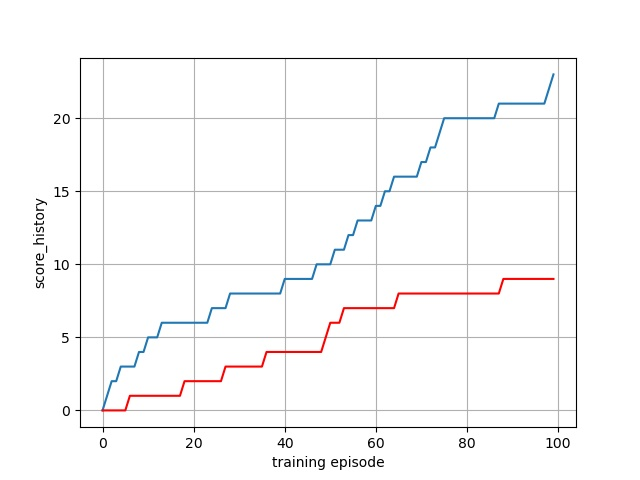
\includegraphics[width=6cm]{score-2-1000-23-9-21-0.jpg}
	}
	\subfigure[2000 episodes]{
		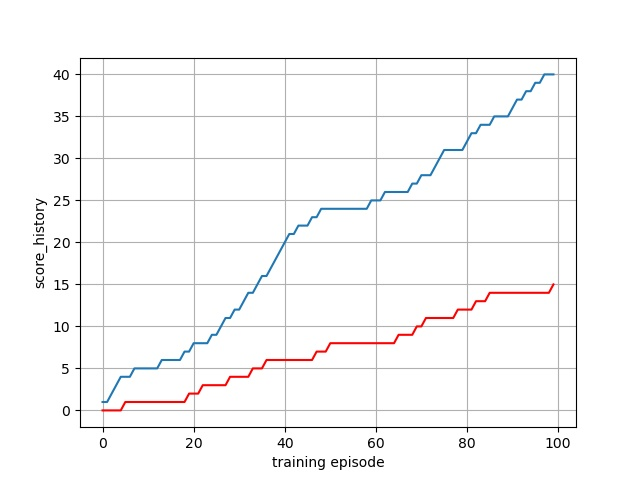
\includegraphics[width=6cm]{score-2-2000-40-15-23-3.jpg}
	}
	\subfigure[4000 episodes]{
		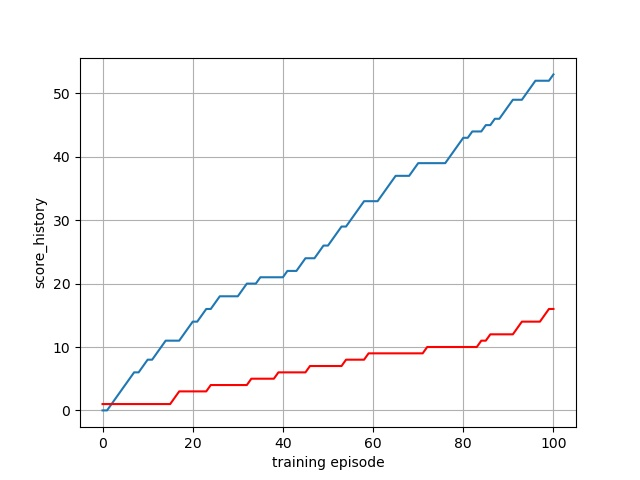
\includegraphics[width=6cm]{score-2-4000-53-16-22-8.jpg}
	}
	\caption{total final scores for 100 round with different training episodes}
\end{figure}

\begin{table}[H]
	\begin{center}
		\begin{tabular}{|c|c|c|c|c|}
			\hline
			episodes  & blue score & red score & blue own goal & red own goal \\ \hline
			0         & 0    & 0    & 0    & 0    \\ \hline
			1000      & 23   & 9    & 21   & 0    \\ \hline
			2000      & 40   & 15   & 23   & 3    \\ \hline
			4000      & 53   & 16   & 22   & 8    \\ \hline
		\end{tabular}
		\caption{Statistics of scores and own goal}
	\end{center}
\end{table}  
 
 From the result, we can see that with more training, the agent becomes more powerful, since both agent could get more scores (no matter if they get the goal by themselves). However, there are too many own goals, especially from the red team. And the diatance of scores are becoming larger and larger. These two phenomenons both show the imbalance of two players during training.

\subsubsection{Different Reward Function}
Then we'd like to find out the difference between our old and new reward function. And the result is below. In each case, the agent is trained with 1000 episodes.

\begin{figure}[htbp]
	\centering
	\subfigure[original reward function]{
		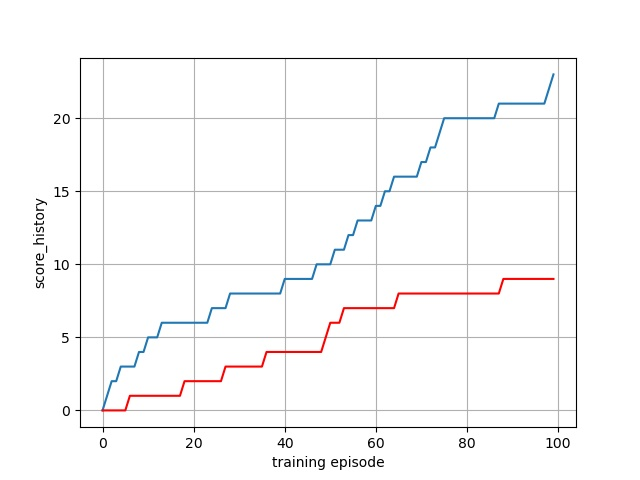
\includegraphics[width=6cm]{score-2-1000-23-9-21-0.jpg}
	}
	\subfigure[new reward function]{
		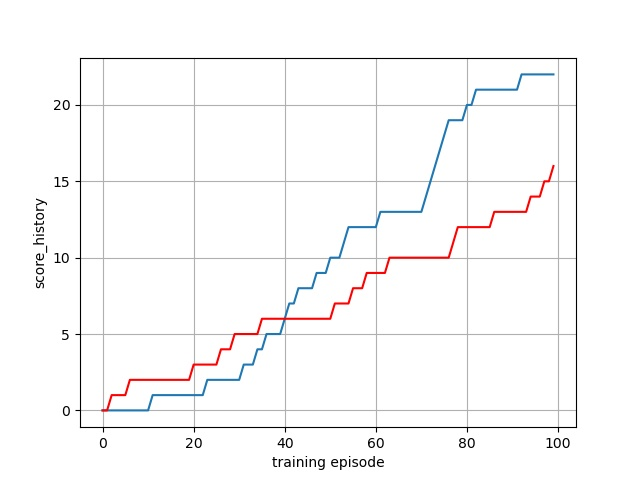
\includegraphics[width=6cm]{score-2-new-1000-22-16-22-5.jpg}
	}
	\caption{total final scores for 100 round with different reward function}
\end{figure}

\begin{table}[H]
	\begin{center}
		\begin{tabular}{|c|c|c|c|c|}
			\hline
			reward  & blue score & red score & blue own goal & red own goal \\ \hline
			original  & 23   & 9    & 21   & 0    \\ \hline
			new       & 22   & 16   & 22   & 5    \\ \hline
		\end{tabular}
		\caption{Statistics of scores and own goal}
	\end{center}
\end{table}

From the comparison we could see that, although no significant difference, but the imbalance between two agents do reduce to a certain extent, approximately 15\%.

%----------------------------------------------------------------------------------------
%	SECTION 5
%----------------------------------------------------------------------------------------

\section{Discussion}

We have to admit that we are far behind our plan in the proposal. We encountered many unexpected difficulty, and we try to solve some of them and try to figure out the reason behind some problem cannot be solved now. In this part, we will discuss these problems we met, and give our opinion and lesson we learnt from them.

\subsection{Slow training speed}
Before we started to train our models, we never reckoned with the slow training speed. The maximum frames we can run per second is about 1000 in a computer with an average CPU, and we train 1 times in 10 frames. This number, 100 times of train in one second, is not a small number at the first look, but it is much slower than what it should have been.

The limitation of the training speed is not the training process itself. The interaction between agents and environment is the limitation. The evidence is that when we use the GPU to do the neural network training, the GPU occupancy is always lower than 2\%, even for a entry level GPU MX350, which really shocks us. Therefore, the game process occupies most of the running time.

Before we found this problem, we through we can use GPU servers provided by CSE Department to accelerate our training, but now we know that the design of our project make it impossible. The lesson we learnt from this problem is that it's better to choose an simple environment, at least a high-performance environment, otherwise the environment may become the barrier to accelerate the training process.

\subsection{Reinforcement Learning is training inefficient}

The part of slow training speed has been discussed in the last section, and the other part of the problem is because of the property of Reinforcement learning. During our training process, we found that the model usually needs thousands of trains to get a perceptible improvement, even in the single player mode, which is a simple environment for even $Q$-learning.

We think this is a universal problem in deep reinforcement learning. Atari games is a standard benchmark for performance of different algorithms, and the exist data show that the the training times for even the best algorithm is in the order of magnitude of 10 million, and those classic algorithms like native-D$Q$N and Double D$Q$N need more rounds(Hessel et al.).

However, CNN is also a popular deep learning algorithm, which is widely used in image recognition. The MNIST is a well-known dataset which is used to train for recognizing handwriting numbers. If we train a CNN model in this dataset, we may not need more than 100 rounds to get 90\% of accuracy, which is much more efficient than deep reinforcement learning.

\subsection{Random seed matters}
Every time  we initialize a new agent, we will initialize the parameter of the network, because we will use the gradient decline to get optimal parameters and different initial values may result in different local optima. In most cases, this will not have a huge negative impact as long as we try several times.
However, in our experiments, randomization will have a huge impact. Agents with the same hyper-parameters can have a huge difference in training speed and  performance after training. This also affects AI versus AI mode, because the power of agents with different initial estimators will be unbalanced during and after training.
The most depressing impact is that it is hard to know if a bad result is caused by incorrect structure or parameters, or caused by bad luck. From previous research, we found that a model set correctly still has a 25\% fail probability(Houthooft et al.). Therefore, we need to train more models with the same parameters to ensure that we can make a fair judgement on our setting. However, slow and ineffective training makes repetition become a time-consuming process.
We guess we can reduce the effect of randomization by giving some prior knowledge, which means we can initialize the network by a user defined function instead of randomizing function. This may help agents to converge in the way we expect.

\subsection{Difficulty in reward functions}

In the result section, we conclude that different reward functions will affect the quality of training. Therefore, the quality of reward function is important for a good training result. However, it is hard to predict the quality of a reward function, since we do not know whether a reward has some side effects. 

For example, in one version of our reward function, we calculate the distance between the ball and current or opponent players. If the difference in these two distances decreases, we will give a reward to the current player, otherwise, a punishment will be given. We thought that this may help player to keep the ball away from the opponent. However, we found that the player may move the ball toward his half and wrongly kick a own goal.

Therefore, we cannot predict how the agent will respond to our reward function, the only things we can do in our project is to try different functions.

\subsection{Overfitting}

In deep reinforcement learning, overfitting may not be a thing we have to avoid, since we will not use the model in other environments. Therefore, overfitting in a specific environment may not affect the accuracy of a model in that environment. However, the problem we met is that the other player is seen as a part of the environment, and an agent will adjust itself according to the other agent.

This overfitting causes 2 problems. First, if there is difference in the performance between the 2 agents, the better one will become better and better as training. The stronger agent will get higher reward because it can always defeat the opponent, so it will become an expert against the other. However, the weaker one cannot get enough positive feedback because the reward is not satisfactory no matter what it does.

The second problem is that a well-trained agent may not perform well when it faces a stranger. The overfitting makes the performance of an agent in a testing environment worse than the training environment. However, our goal is to train an agent to play the game, instead of beating a specific agent.
%----------------------------------------------------------------------------------------
%	BIBLIOGRAPHY
%----------------------------------------------------------------------------------------

\begin{thebibliography}{99}
	\bibitem{ref1}Silver, David, et al. "Mastering the game of Go with deep neural networks and tree search." nature 529.7587 (2016): 484-489.

	\bibitem{ref2}Mnih, Volodymyr, et al. "Playing atari with deep reinforcement learning." arXiv preprint arXiv:1312.5602 (2013).

	\bibitem{ref3}Berner, Christopher, et al. "Dota 2 with large scale deep reinforcement learning." arXiv preprint arXiv:1912.06680 (2019).

    \bibitem{ref4}Zoph, Barret, and Quoc V. Le. "Neural architecture search with reinforcement learning." arXiv preprint arXiv:1611.01578 (2016).

    \bibitem{ref5}Mnih, Volodymyr, et al. "Human-level control through deep reinforcement learning." nature 518.7540 (2015): 529-533.

    \bibitem{ref6}Zhou. "Reinforcement Learning Methods and Tutorials" https://github.com/MorvanZhou/Reinforcement-learning-with-tensorflow.

    \bibitem{ref7}Wang SC. (2003) Artificial Neural Network. In: Interdisciplinary Computing in Java Programming. The Springer International Series in Engineering and Computer Science, vol 743. Springer, Boston, MA.

    \bibitem{ref8}Hessel, Matteo, et al. "Rainbow: Combining improvements in deep reinforcement learning." Proceedings of the AAAI Conference on Artificial Intelligence. Vol. 32. No. 1. 2018.

    \bibitem{ref9}Houthooft, Rein, et al. "Vime: Variational information maximizing exploration." arXiv preprint arXiv:1605.09674 (2016).
\end{thebibliography}
%----------------------------------------------------------------------------------------


\end{document}